\documentclass{article}
\usepackage{tikz}
\usepackage{pgfplots}
\pgfplotsset{compat=1.16}

\begin{document}

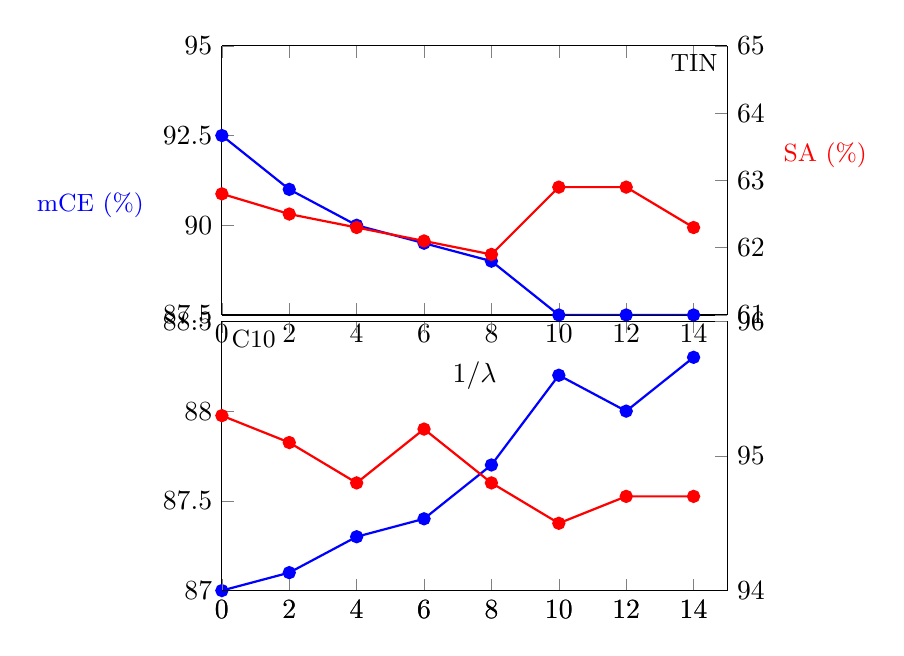
\begin{tikzpicture}
\begin{axis}[
    width=8cm,
    height=5cm,
    xmin=0, xmax=15,
    ymin=87.5, ymax=95,
    ylabel={\textcolor{blue}{mCE (\%)}},
    ylabel style={font=\small, rotate=-90, yshift=-9pt},
    axis y line*=left,
    ytick={87.5, 90, 92.5, 95},
    xlabel={$1/\lambda$},
    title={TIN},
    title style={font=\small, yshift=-0.2cm, anchor=north east, at={(1,1)}},
    legend style={at={(0.97,0.97)}, anchor=north east, font=\small},
]

% Blue line (mCE)
\addplot[thick, blue, mark=*, mark size=2pt] coordinates {
    (0, 92.5)
    (2, 91)
    (4, 90)
    (6, 89.5)
    (8, 89)
    (10, 87.5)
    (12, 87.5)
    (14, 87.5)
};

% Create a second y-axis
\end{axis}

\begin{axis}[
    width=8cm,
    height=5cm,
    xmin=0, xmax=15,
    ymin=61, ymax=65,
    ylabel={\textcolor{red}{SA (\%)}},
    ylabel style={font=\small, rotate=-90, yshift=9pt},
    axis y line*=right,
    axis x line=none,
    ytick={61, 62, 63, 64, 65},
]

% Red line (SA)
\addplot[thick, red, mark=*, mark size=2pt] coordinates {
    (0, 62.8)
    (2, 62.5)
    (4, 62.3)
    (6, 62.1)
    (8, 61.9)
    (10, 62.9)
    (12, 62.9)
    (14, 62.3)
};

\end{axis}

\begin{axis}[
    width=8cm,
    height=5cm,
    xmin=0, xmax=15,
    ymin=87, ymax=88.5,
    axis y line*=left,
    ytick={87, 87.5, 88, 88.5},
    xlabel={},
    title={C10},
    title style={font=\small, yshift=-0.2cm, anchor=north west, at={(0,1)}},
    yshift=-3.5cm,
]

% Blue line (RA)
\addplot[thick, blue, mark=*, mark size=2pt] coordinates {
    (0, 87)
    (2, 87.1)
    (4, 87.3)
    (6, 87.4)
    (8, 87.7)
    (10, 88.2)
    (12, 88)
    (14, 88.3)
};

\end{axis}

\begin{axis}[
    width=8cm,
    height=5cm,
    xmin=0, xmax=15,
    ymin=94, ymax=96,
    axis y line*=right,
    axis x line*=bottom,
    ytick={94, 95, 96},
    yshift=-3.5cm,
]

% Red line (SA)
\addplot[thick, red, mark=*, mark size=2pt] coordinates {
    (0, 95.3)
    (2, 95.1)
    (4, 94.8)
    (6, 95.2)
    (8, 94.8)
    (10, 94.5)
    (12, 94.7)
    (14, 94.7)
};

\end{axis}
\end{tikzpicture}

\end{document}